\chapter{Числени тестове на алгоритмите в системата за прогнозиране}

Програмният модул, използван за извършването на представените експерименти е изваден, като изолиран подмодул на софтуерната разработка в настоящия дисертационен труд. Кодът се тества самостоятелно, за да се отстранят ефектите от асинхронно изпълнение, във фонов режим, породен от организацията на изпълнението в операционната система Android OS. Работата на изолираните подмодули в цялостната реализация на софтуера не би позволила ефективно измерване на ангажираните изчислителни ресурси и използваното изчислително време. Също така, измерване на производителността върху мобилни устройства е значително по-ненадеждно, отколкото при настолни компютърни системи. 

Прогнозирането в мобилното приложение от страната на клиента се извършва с трислоен перцептрон. Времевият ред се разбива на двойки минало-бъдеще, които съставляват обучаващите примери. Разделението на минал и бъдещ период е условно. Практически, цялата информация е от данни в миналото. С пълзящ прозорец, условното разделяне се получава за минали стойности и стойности в бъдещия момент, спрямо условния разделител. Разполагайки с тренировъчни примери, процесът по обучението на трислойния перцептрон е свързан с търсене на тегла, водещи до минимизирането на общата грешка, която мрежата допуска. В системата са реализирани два начина за търсене на оптимални тегла – точни градиентни и евристични. Двата начина се активират на случаен принцип с равна вероятност (Листинг \ref{list0020}).

\begin{lstlisting}[caption=Превключване на алгоритмите за обучение, language=Java, basicstyle=\tiny, label=list0020]
/* Switch between gradient and evolutionry algorithm. */
if (PRNG.nextBoolean() == true) {
	/* Gradient-based optimization. */
} else {
	/* Evolutionary optimization. */
}
\end{lstlisting}

Ефективността на двата начина за оптимизиране на теглата се подлага на изследване, като алгоритмите се изолират да работят самостоятелно, извън общата работа на системата. 

\section{Точни числени алгоритми}

Encog Machine Learning Framework поддържа множество алгоритми за обучение на изкуствени невронни мрежи, като от тях са избрани пет точни числени алгоритъма (Листинг \ref{list0021}).

\begin{lstlisting}[caption=Набор от точни числени алгоритми, language=Java, basicstyle=\tiny, label=list0021]
/* Selection of gradient-based training. */
Propagation[] propagations = {
	new Backpropagation((BasicNetwork) network.clone(), examples),
	new ResilientPropagation((BasicNetwork) network.clone(), examples),
	new QuickPropagation((BasicNetwork) network.clone(), examples),
	new ScaledConjugateGradient((BasicNetwork) network.clone(), examples),
	new ManhattanPropagation((BasicNetwork) network.clone(), examples, PRNG.nextDouble())
};
\end{lstlisting}

Класът Backpropagation реализира традиционният алгоритъм за обратно разпространение на грешката, който разчита на частни производни. При алгоритъма за обратно разпространение на грешката съществува проблем с магнитута на производните, когато те дават твърде големи или твърде малки стойности. Втори недостатък на алгоритъма за обратно разпространение на грешката е, че параметърът за научаване (learning rate) е една единствена стойност за цялата мрежа. 

Класът ResilientPropagation реализира подобрение на алгоритъма за обратно разпространение на грешката, като въвежда коефициент за обновление (update value) на всяка връзка между два неврона. Значително предимство е, че конкретните стойности за коефициента на обновление се определят автоматично и не е нужна човешка намеса. Това е водеща разлика от класическия алгоритъм за обратно разпространение на грешката, където параметъра за научаване е предварително дефиниран, и то ръчно. 

Класът QuickPropagation внася подобрение на алгоритъма за обратно разпространение на грешката, като използва Нютон методите. Състои се в квадратична апроксимация на последващите стъпки в градиента. По този начин общо допуснатата от изкуствената невронна мрежа грешка се представя като парабола, чието дъно би било минимум за общата допусната грешка. Недостатък при тази модификация на алгоритъма за обратно разпространение на грешката е, че поведението на изкуствената невронна мрежа може да се окаже хаотично, при големите стъпки за обновление на теглата. 

ScaledConjugateGradient класът реализира обучение на принципа на линейните посоки, като не прави всеки път линейно търсене. Ако бъде правено линейно търсене на всяка итерация, това би направило обучението твърде неефективно, по отношение на изчислително време. Алгоритъмът се прилага за изкуствени невронни мрежи, в които функциите имат дефинирани производни. 

ManhattanPropagation класът се опитва да въведе подобрение в класическото обратно разпространение на грешката, като единствено използва знака на производната, но не и нейния магнитут. Корекцията на теглата се извършва с предварително зададена стойност. Тази предварително зададена стойност се определя експериментално. Манхатън обучението може да се смята за опростен вариант на еластиочното (Resilient) обучение.

При равни други условия се стартира обучение с всеки един от алгоритмите, като се отчитат броя оптимизационни цикли и обща допусната грешка от изкуствената невронна мрежа (Листинг \ref{list0022}).\pagebreak

\begin{lstlisting}[caption=Експериментална проверка на точните числени алгоритми, language=Java, basicstyle=\tiny, label=list0022]
System.out.println("Experiment start.");
for (Propagation p : propagations) {
    System.out.println("" + p.getClass().getName());
    long loop = 0;
    long second = 0;
    long time = System.currentTimeMillis();
    long start = System.currentTimeMillis();
    while (p.isTrainingDone() == false && System.currentTimeMillis()-start < 1*60*1000) {
        loop++;
        p.iteration();
        if(System.currentTimeMillis()-time > 1000) {
            second++;
            System.out.println(second + "\t" + loop + "\t" + p.getError());
            time = System.currentTimeMillis();
        }
    }
    p.finishTraining();
}
System.out.println("Experiment end.");
\end{lstlisting}

Експериментите са извършени с два комплекта данни – базова форма на времеви ред, следваща синус функция (Фиг. \ref{fig0072}) и цена на дигиталната валута биткойн в щатски долари (Фиг. \ref{fig0083}). 

\subsection{Синус функция}

\begin{figure}[H]
  \centering
  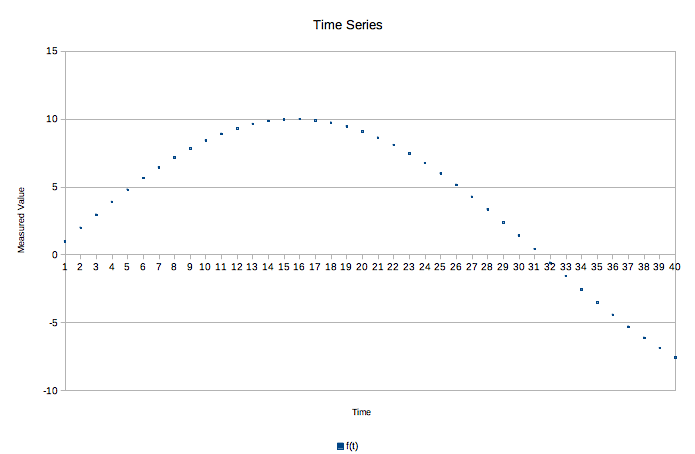
\includegraphics[width=0.8\linewidth]{fig0072.png}
  \caption{Времеви ред следващ синус функция}
\label{fig0072}
\end{figure}

%\begin{figure}[H]
%  \centering
%  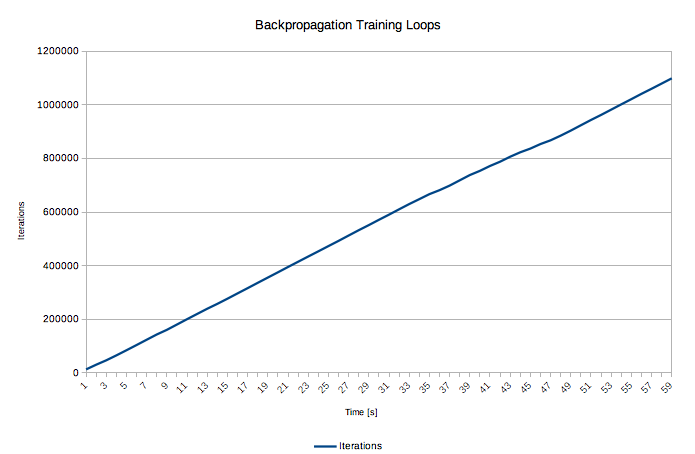
\includegraphics[width=0.8\linewidth]{fig0073.png}
%  \caption{Backpropagation брой тренировъчни цикли}
%\label{fig0073}
%\end{figure}
%
%\begin{figure}[H]
%  \centering
%  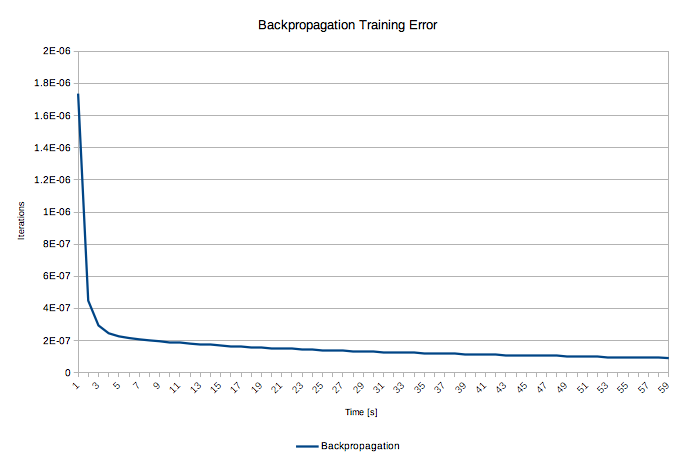
\includegraphics[width=0.8\linewidth]{fig0074.png}
%  \caption{Backpropagation обща грешка на изкуствената невронна мрежа}
%\label{fig0074}
%\end{figure}
%
%\begin{figure}[H]
%  \centering
%  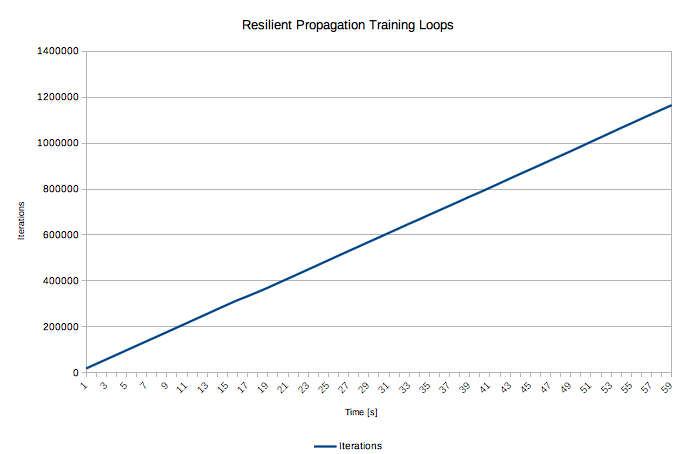
\includegraphics[width=0.8\linewidth]{fig0075.png}
%  \caption{ResilientPropagation брой тренировъчни цикли}
%\label{fig0075}
%\end{figure}
%
%\begin{figure}[H]
%  \centering
%  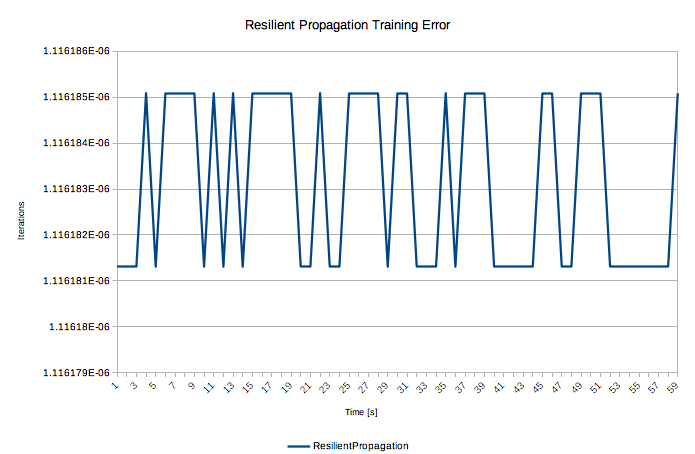
\includegraphics[width=0.8\linewidth]{fig0076.png}
%  \caption{ResilientPropagation обща грешка на изкуствената невронна мрежа}
%\label{fig0076}
%\end{figure}
%
%\begin{figure}[H]
%  \centering
%  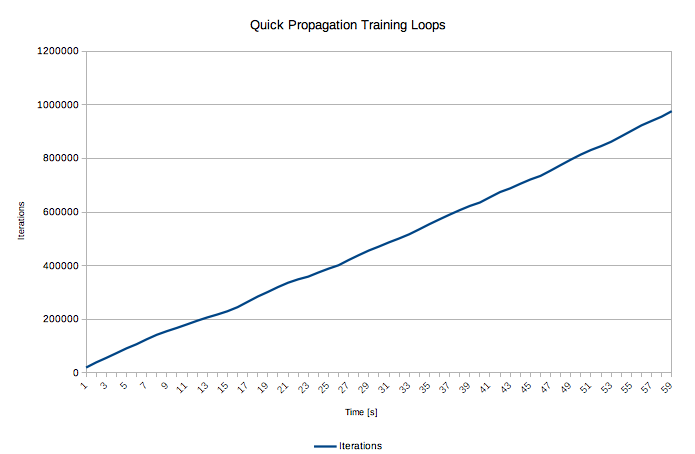
\includegraphics[width=0.8\linewidth]{fig0077.png}
%  \caption{QuickPropagation брой тренировъчни цикли}
%\label{fig0077}
%\end{figure}
%
%\begin{figure}[H]
%  \centering
%  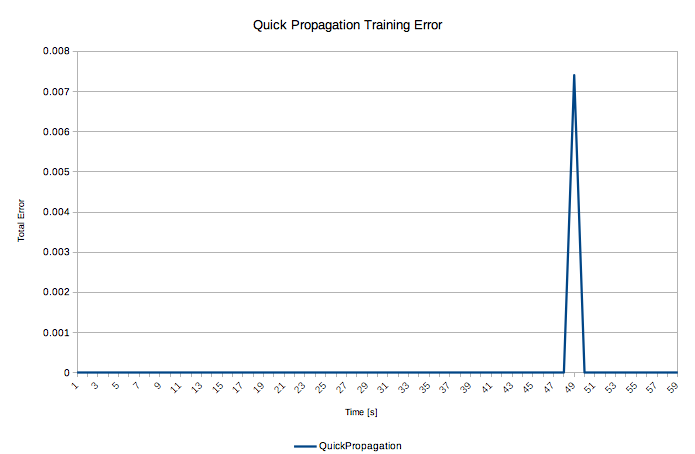
\includegraphics[width=0.8\linewidth]{fig0078.png}
%  \caption{QuickPropagation обща грешка на изкуствената невронна мрежа}
%\label{fig0078}
%\end{figure}
%
%\begin{figure}[H]
%  \centering
%  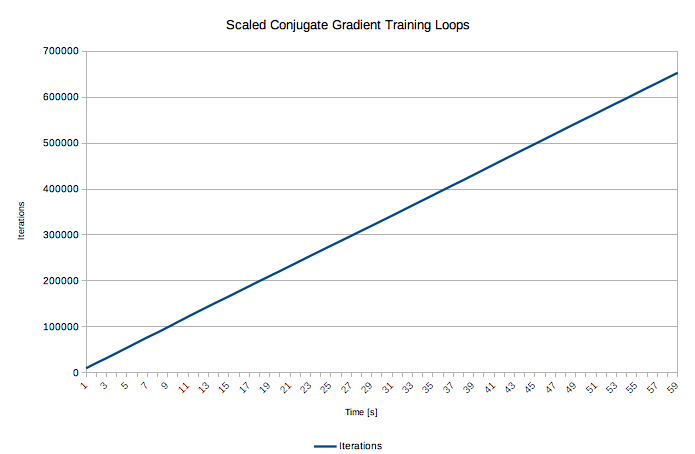
\includegraphics[width=0.8\linewidth]{fig0079.png}
%  \caption{ScaledConjugateGradient брой тренировъчни цикли}
%\label{fig0079}
%\end{figure}
%
%\begin{figure}[H]
%  \centering
%  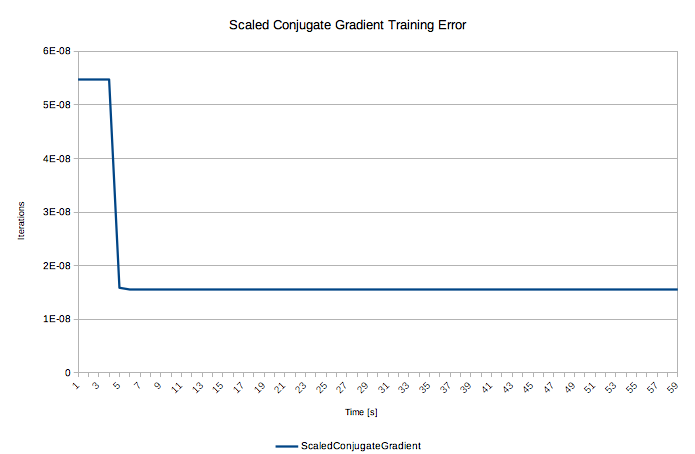
\includegraphics[width=0.8\linewidth]{fig0080.png}
%  \caption{ScaledConjugateGradient обща грешка на изкуствената невронна мрежа}
%\label{fig0080}
%\end{figure}
%
%\begin{figure}[H]
%  \centering
%  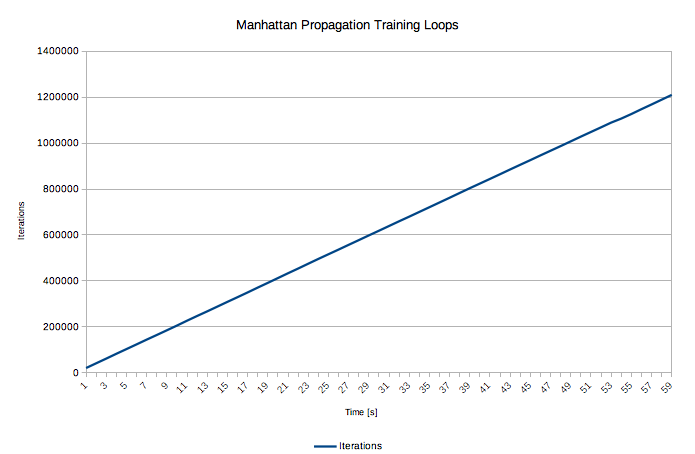
\includegraphics[width=0.8\linewidth]{fig0081.png}
%  \caption{ManhattanPropagation брой тренировъчни цикли}
%\label{fig0081}
%\end{figure}
%
%\begin{figure}[H]
%  \centering
%  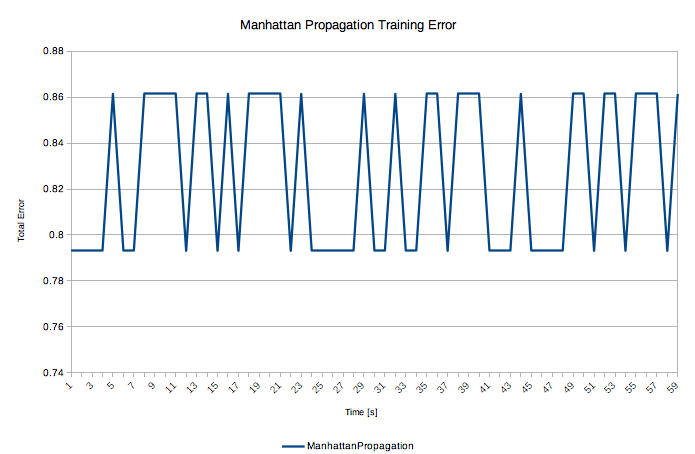
\includegraphics[width=0.8\linewidth]{fig0082.png}
%  \caption{ManhattanPropagation обща грешка на изкуствената невронна мрежа}
%\label{fig0082}
%\end{figure}
%
\begin{figure}[H]
  \begin{subfigure}{0.49\textwidth}
  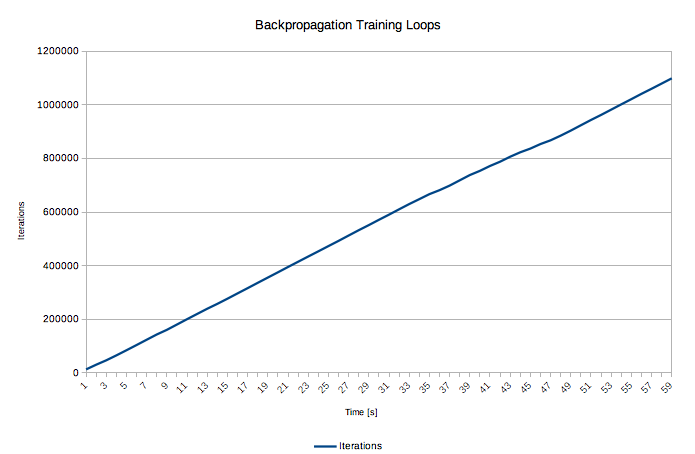
\includegraphics[width=\linewidth]{fig0073.png}
  \subcaption{\tiny Брой тренировъчни цикли}
  \label{fig0073}
  \end{subfigure}
  \begin{subfigure}{0.49\textwidth}
  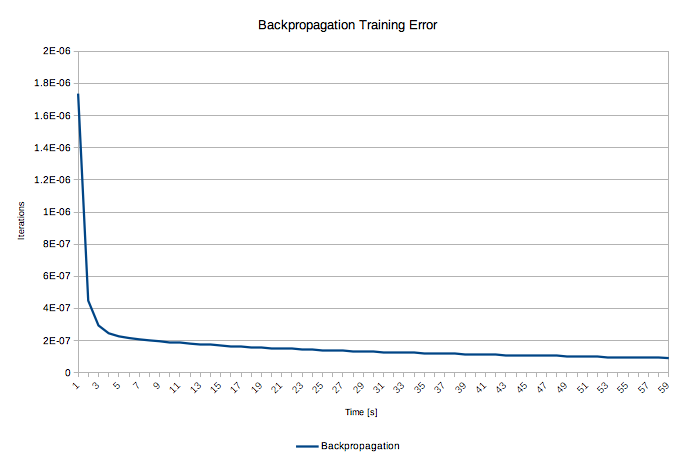
\includegraphics[width=\linewidth]{fig0074.png}
  \subcaption{\tiny Обща грешка допусната от ИНМ}
  \label{fig0074}
  \end{subfigure}
  \caption{Backpropagation}
\end{figure}

\begin{figure}[H]
  \begin{subfigure}{0.49\textwidth}
  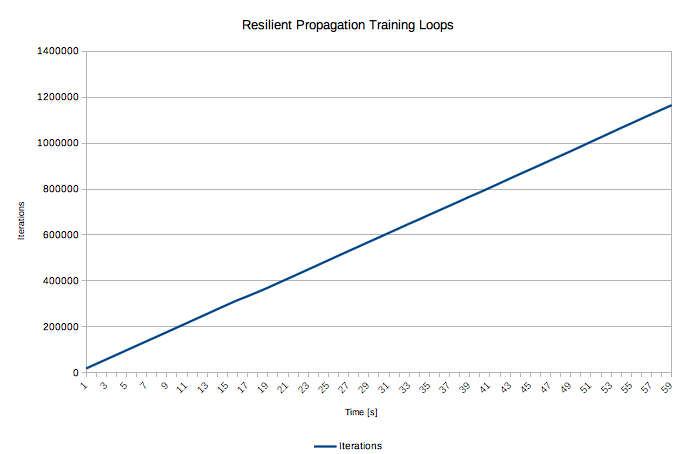
\includegraphics[width=\linewidth]{fig0075.png}
  \subcaption{\tiny Брой тренировъчни цикли}
  \label{fig0075}
  \end{subfigure}
  \begin{subfigure}{0.49\textwidth}
  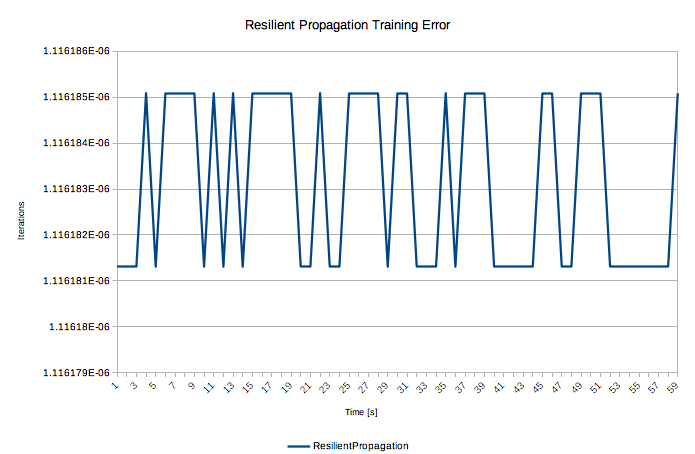
\includegraphics[width=\linewidth]{fig0076.png}
  \subcaption{\tiny Обща грешка допусната от ИНМ}
  \label{fig0076}
  \end{subfigure}
  \caption{ResilientPropagation}
\end{figure}

\begin{figure}[H]
  \begin{subfigure}{0.49\textwidth}
  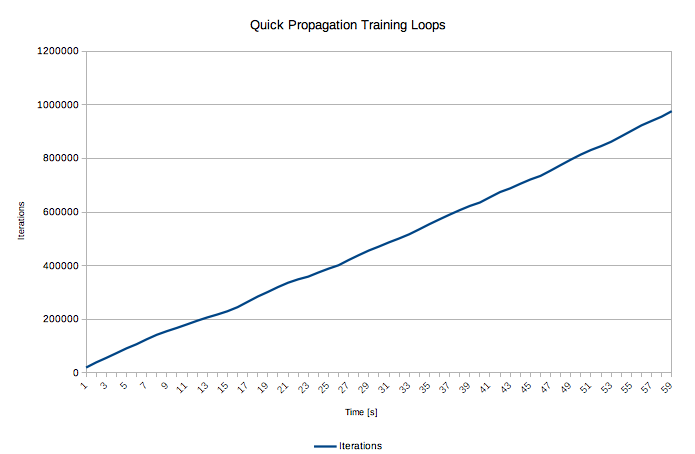
\includegraphics[width=\linewidth]{fig0077.png}
  \subcaption{\tiny Брой тренировъчни цикли}
  \label{fig0077}
  \end{subfigure}
  \begin{subfigure}{0.49\textwidth}
  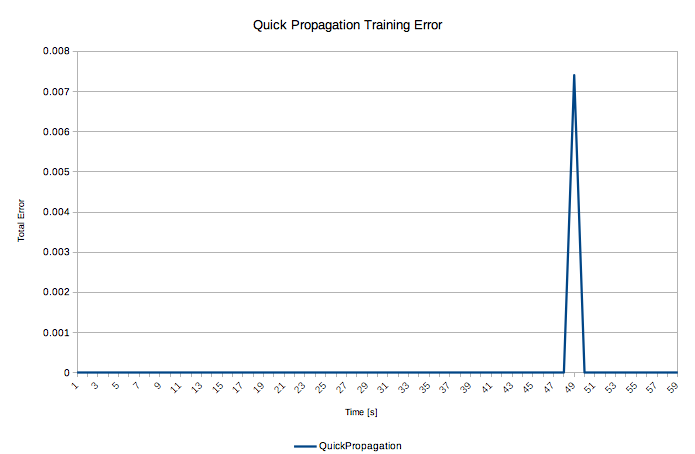
\includegraphics[width=\linewidth]{fig0078.png}
  \subcaption{\tiny Обща грешка допусната от ИНМ}
  \label{fig0078}
  \end{subfigure}
  \caption{QuickPropagation}
\end{figure}

\begin{figure}[H]
  \begin{subfigure}{0.49\textwidth}
  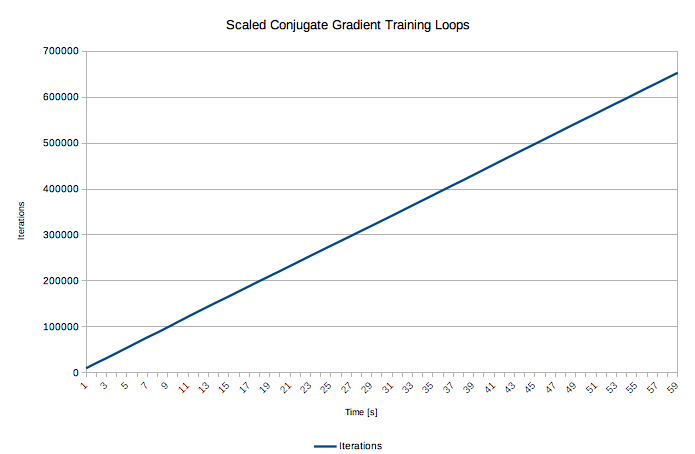
\includegraphics[width=\linewidth]{fig0079.png}
  \subcaption{\tiny Брой тренировъчни цикли}
  \label{fig0079}
  \end{subfigure}
  \begin{subfigure}{0.49\textwidth}
  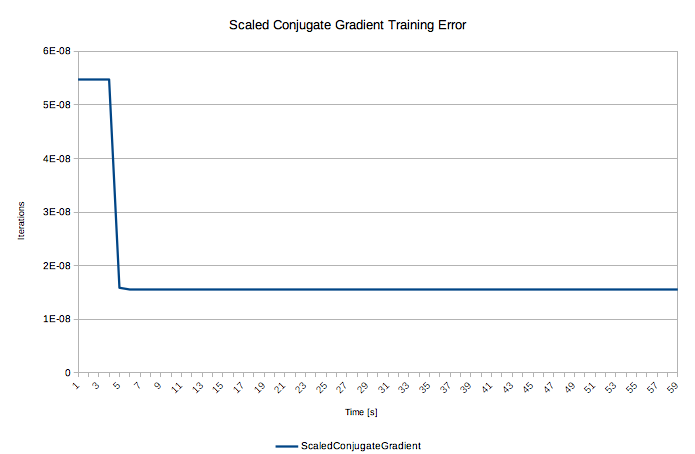
\includegraphics[width=\linewidth]{fig0080.png}
  \subcaption{\tiny Обща грешка допусната от ИНМ}
  \label{fig0080}
  \end{subfigure}
  \caption{ScaledConjugateGradient}
\end{figure}

\begin{figure}[H]
  \begin{subfigure}{0.49\textwidth}
  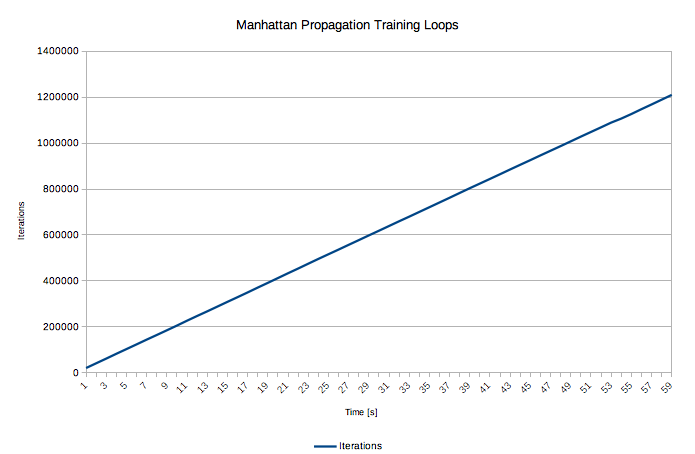
\includegraphics[width=\linewidth]{fig0081.png}
  \subcaption{\tiny Брой тренировъчни цикли}
  \label{fig0081}
  \end{subfigure}
  \begin{subfigure}{0.49\textwidth}
  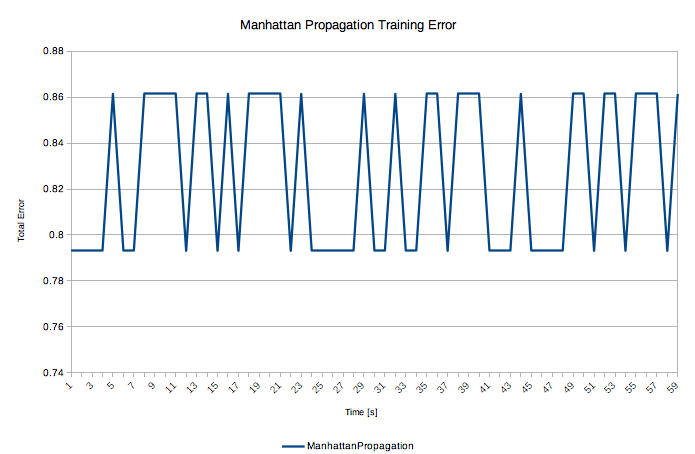
\includegraphics[width=\linewidth]{fig0082.png}
  \subcaption{\tiny Обща грешка допусната от ИНМ}
  \label{fig0082}
  \end{subfigure}
  \caption{ManhattanPropagation}
\end{figure}

\newpage

\subsection{Цена на биткойн}

\begin{figure}[H]
  \centering
  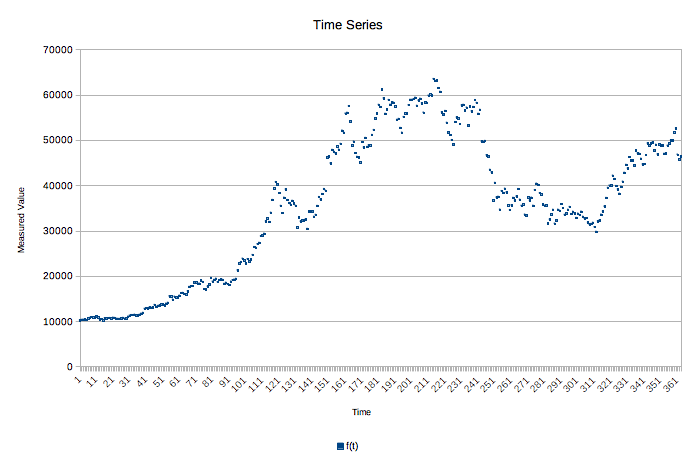
\includegraphics[width=0.8\linewidth]{fig0083.png}
  \caption{Времеви ред с цената на биткойн}
\label{fig0083}
\end{figure}

%\begin{figure}[H]
%  \centering
%  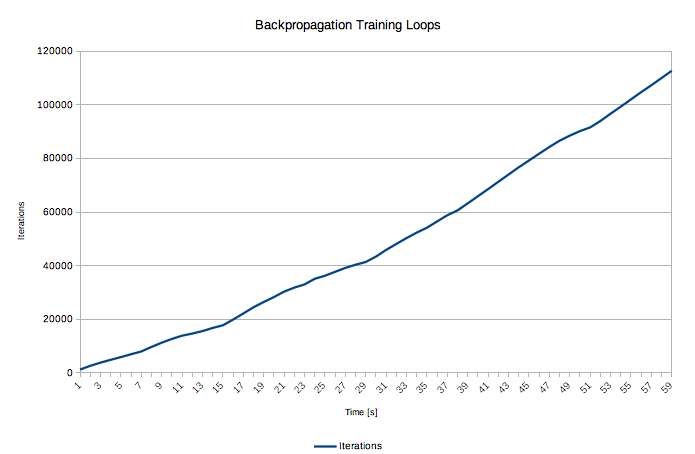
\includegraphics[width=0.8\linewidth]{fig0084.png}
%  \caption{Backpropagation брой тренировъчни цикли}
%\label{fig0084}
%\end{figure}
%
%\begin{figure}[H]
%  \centering
%  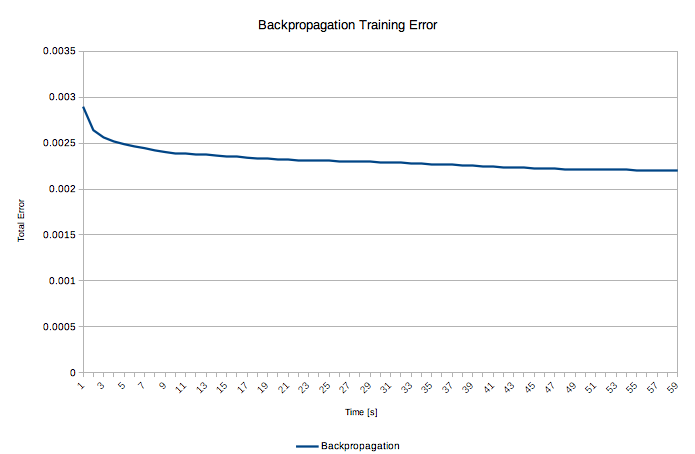
\includegraphics[width=0.8\linewidth]{fig0085.png}
%  \caption{Backpropagation обща грешка на изкуствената невронна мрежа}
%\label{fig0085}
%\end{figure}
%
%\begin{figure}[H]
%  \centering
%  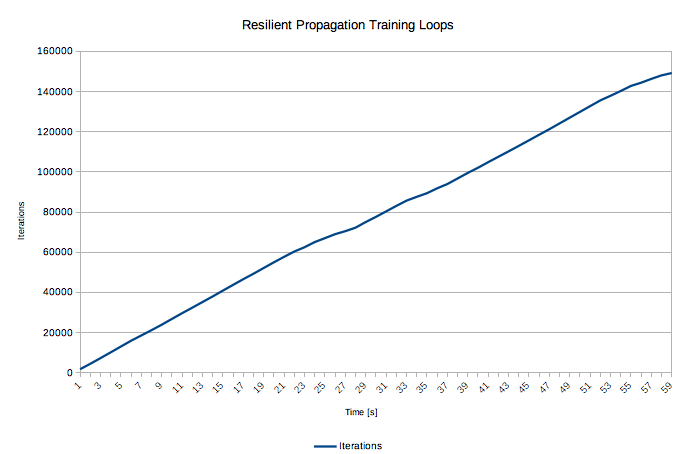
\includegraphics[width=0.8\linewidth]{fig0086.png}
%  \caption{ResilientPropagation брой тренировъчни цикли}
%\label{fig0086}
%\end{figure}
%
%\begin{figure}[H]
%  \centering
%  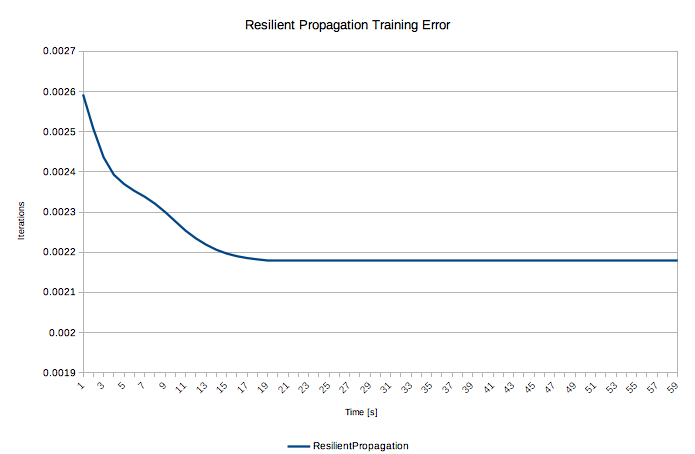
\includegraphics[width=0.8\linewidth]{fig0087.png}
%  \caption{ResilientPropagation обща грешка на изкуствената невронна мрежа}
%\label{fig0087}
%\end{figure}
%
%\begin{figure}[H]
%  \centering
%  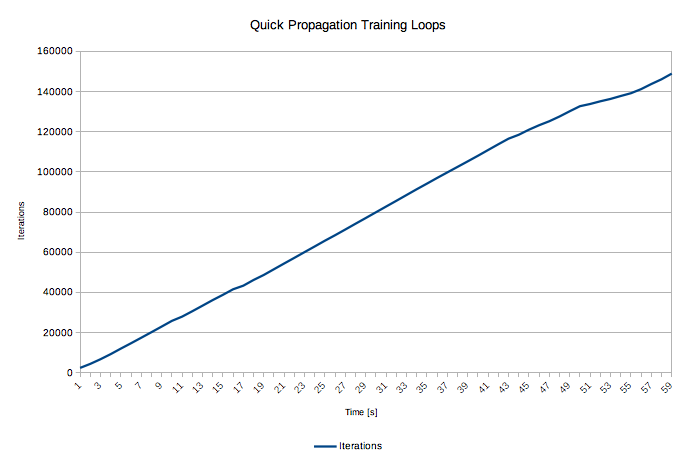
\includegraphics[width=0.8\linewidth]{fig0088.png}
%  \caption{QuickPropagation брой тренировъчни цикли}
%\label{fig0088}
%\end{figure}
%
%\begin{figure}[H]
%  \centering
%  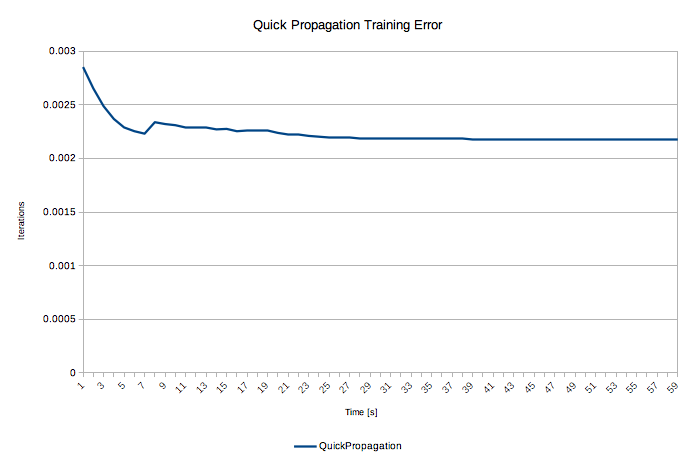
\includegraphics[width=0.8\linewidth]{fig0089.png}
%  \caption{QuickPropagation обща грешка на изкуствената невронна мрежа}
%\label{fig0089}
%\end{figure}
%
%\begin{figure}[H]
%  \centering
%  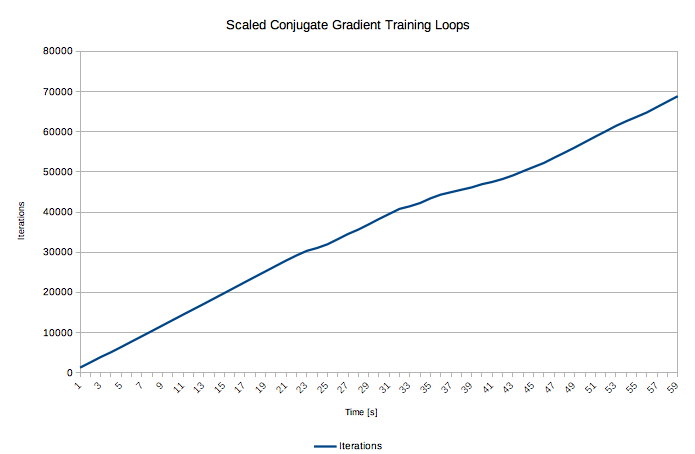
\includegraphics[width=0.8\linewidth]{fig0090.png}
%  \caption{ScaledConjugateGradient брой тренировъчни цикли}
%\label{fig0090}
%\end{figure}
%
%\begin{figure}[H]
%  \centering
%  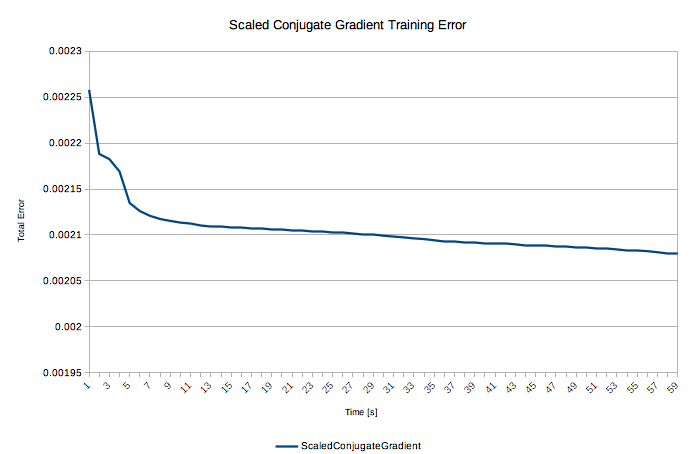
\includegraphics[width=0.8\linewidth]{fig0091.png}
%  \caption{ScaledConjugateGradient обща грешка на изкуствената невронна мрежа}
%\label{fig0091}
%\end{figure}
%
%\begin{figure}[H]
%  \centering
%  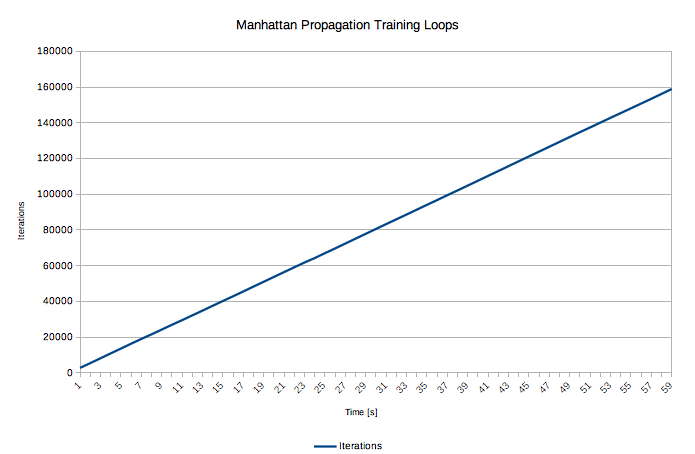
\includegraphics[width=0.8\linewidth]{fig0092.png}
%  \caption{ManhattanPropagation брой тренировъчни цикли}
%\label{fig0092}
%\end{figure}
%
%\begin{figure}[H]
%  \centering
%  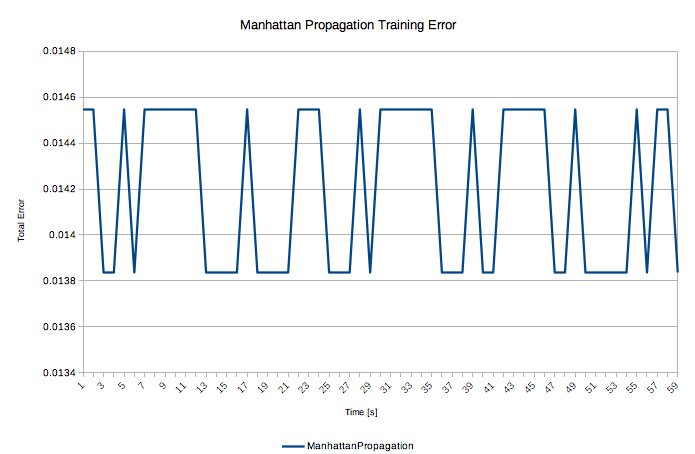
\includegraphics[width=0.8\linewidth]{fig0093.png}
%  \caption{ManhattanPropagation обща грешка на изкуствената невронна мрежа}
%\label{fig0093}
%\end{figure}
%
\begin{figure}[H]
  \begin{subfigure}{0.49\textwidth}
  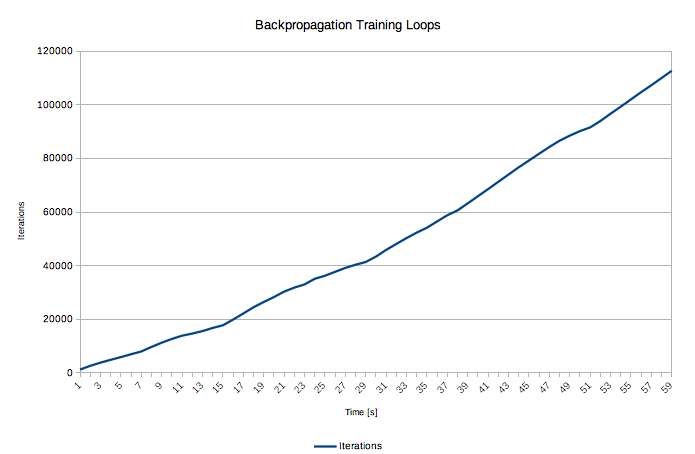
\includegraphics[width=\linewidth]{fig0084.png}
  \subcaption{\tiny Брой тренировъчни цикли}
  \label{fig0084}
  \end{subfigure}
  \begin{subfigure}{0.49\textwidth}
  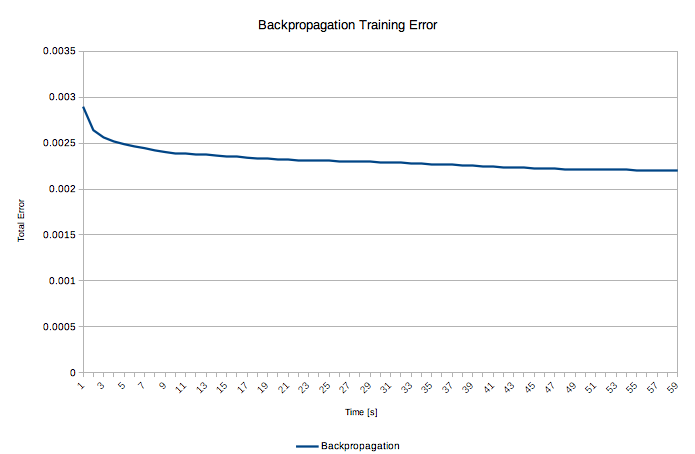
\includegraphics[width=\linewidth]{fig0085.png}
  \subcaption{\tiny Обща грешка допусната от ИНМ}
  \label{fig0085}
  \end{subfigure}
  \caption{Backpropagation}
\end{figure}

\begin{figure}[H]
  \begin{subfigure}{0.49\textwidth}
  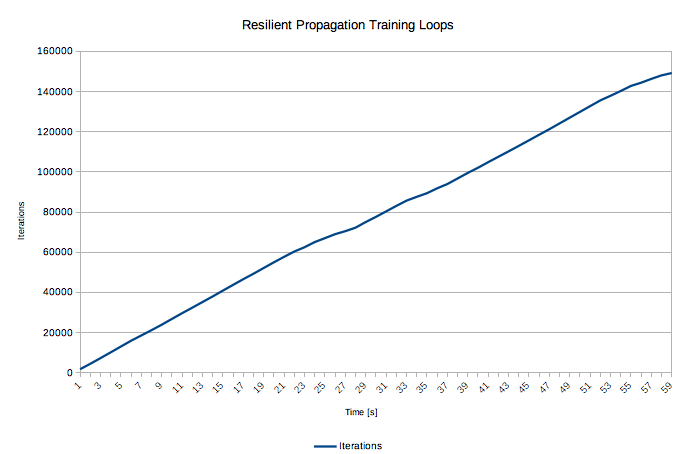
\includegraphics[width=\linewidth]{fig0086.png}
  \subcaption{\tiny Брой тренировъчни цикли}
  \label{fig0086}
  \end{subfigure}
  \begin{subfigure}{0.49\textwidth}
  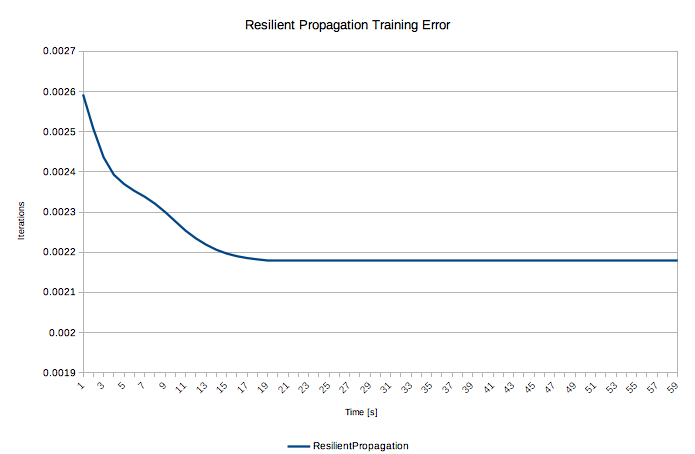
\includegraphics[width=\linewidth]{fig0087.png}
  \subcaption{\tiny Обща грешка допусната от ИНМ}
  \label{fig0087}
  \end{subfigure}
  \caption{ResilientPropagation}
\end{figure}

\begin{figure}[H]
  \begin{subfigure}{0.49\textwidth}
  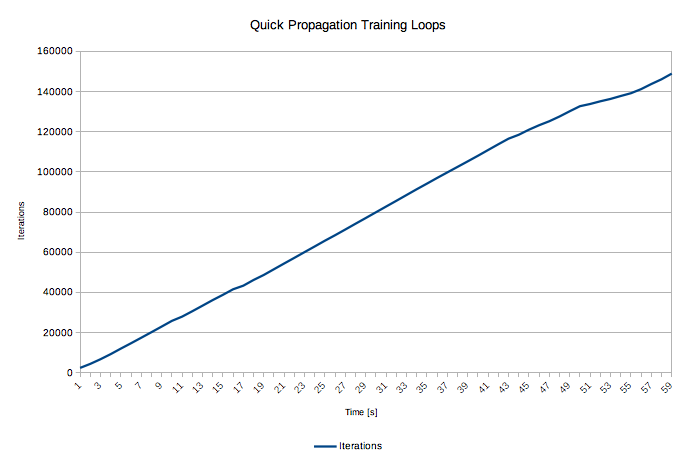
\includegraphics[width=\linewidth]{fig0088.png}
  \subcaption{\tiny Брой тренировъчни цикли}
  \label{fig0088}
  \end{subfigure}
  \begin{subfigure}{0.49\textwidth}
  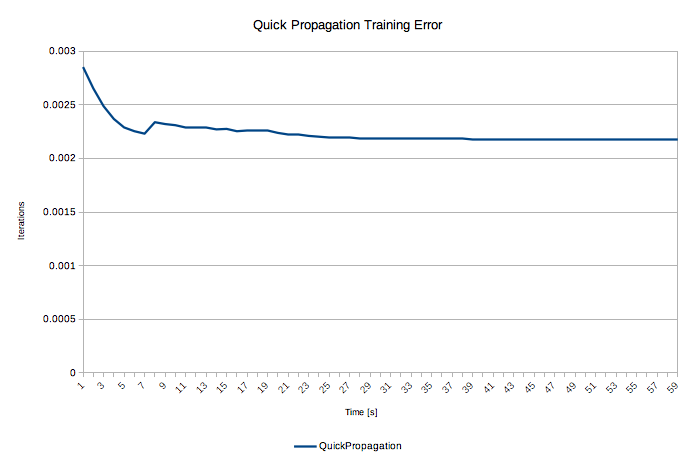
\includegraphics[width=\linewidth]{fig0089.png}
  \subcaption{\tiny Обща грешка допусната от ИНМ}
  \label{fig0089}
  \end{subfigure}
  \caption{QuickPropagation}
\end{figure}

\begin{figure}[H]
  \begin{subfigure}{0.49\textwidth}
  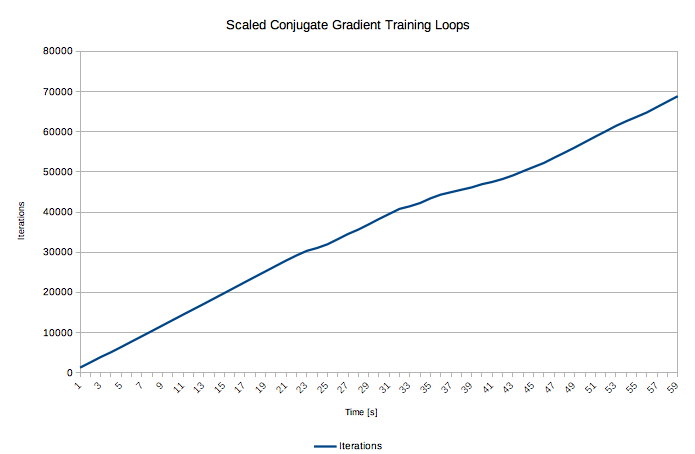
\includegraphics[width=\linewidth]{fig0090.png}
  \subcaption{\tiny Брой тренировъчни цикли}
  \label{fig0090}
  \end{subfigure}
  \begin{subfigure}{0.49\textwidth}
  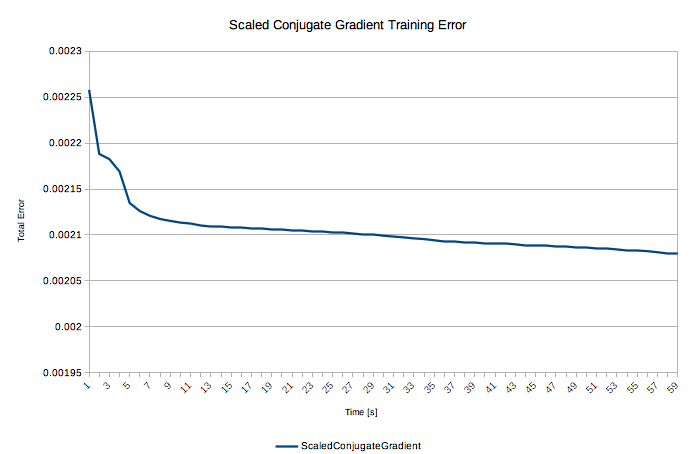
\includegraphics[width=\linewidth]{fig0091.png}
  \subcaption{\tiny Обща грешка допусната от ИНМ}
  \label{fig0091}
  \end{subfigure}
  \caption{ScaledConjugateGradient}
\end{figure}

\begin{figure}[H]
  \begin{subfigure}{0.49\textwidth}
  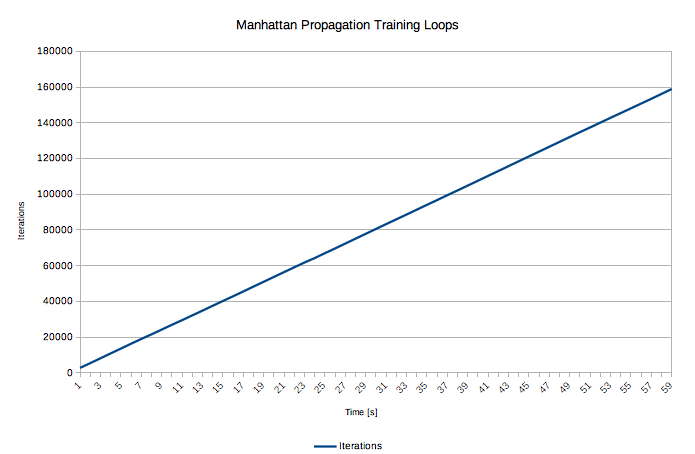
\includegraphics[width=\linewidth]{fig0092.png}
  \subcaption{\tiny Брой тренировъчни цикли}
  \label{fig0092}
  \end{subfigure}
  \begin{subfigure}{0.49\textwidth}
  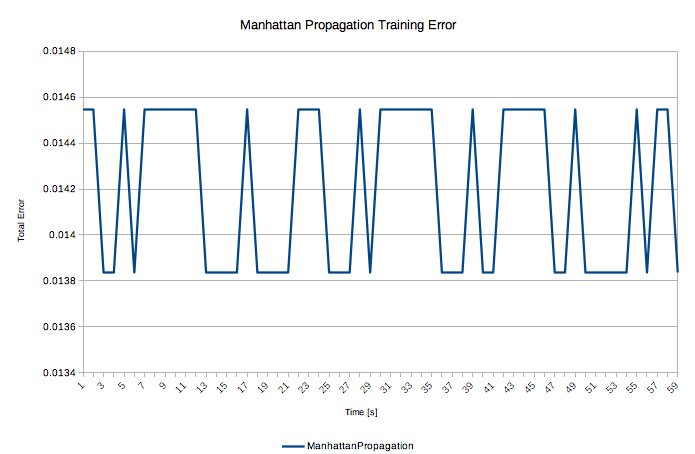
\includegraphics[width=\linewidth]{fig0093.png}
  \subcaption{\tiny Обща грешка допусната от ИНМ}
  \label{fig0093}
  \end{subfigure}
  \caption{ManhattanPropagation}
\end{figure}

\subsection{Анализ на ефективността}

Резултатите (Фиг. \ref{fig0073}-\ref{fig0082}) от проведените експерименти показват, че при точните числени алгоритми класическият алгоритъмът с обратно разпространение на грешката дава най-добра ефективност, за времеви ред с относително опростена структура. При времеви ред със значително по-сложна структура, еластичното (Resilient) обучение е с най-добра ефективност (Фиг. \ref{fig0084}-\ref{fig0093}). При точни числени алгоритми и времеви ред с проста и сложна структура, Манхатън обучението показва най-слаба ефективност. Допуснатата грешка при този вид обучение е поне десет пъти по-голяма в сравнение с най-добре представящите се алгоритми. 

\section{Еволюционни алгоритми}

MOEA Framework поддържа множество евристични оптимизационни алгоритми, като основното предназначение на тази софтуерна библиотека е многокритериална оптимизация. В добавка към многокритериалната оптимизация, библиотеката поддържа и малка група еднокритериални алгоритми. От еднокритериалните алгоритми са избрани еволюционна стратегия (Evolution Strategy), генетичен алгоритъм (Genetic Algorithm) и еволюция на разликите (Differential Evolution). И трите алгоритъма организират търсенето на решение под формата на популация. Популацията от решения еволюира и във всяко следващо поколение очакването е да се появяват решения все по-близки до глобален оптимум (единственият или някой от оптимумите, ако са повече от един). Трите алгоритъма отново са изпълнени за двата комплекта данни - базова форма на времеви ред, следваща синус функция (Фиг. \ref{fig0072}) и цена на дигиталната валута биткойн в щатски долари (Фиг. \ref{fig0083}).

Използва се същата топология на изкуствена невронна мрежа, но вместо градиентен алгоритми, теглата на мрежата се ползват за инициализиране на начална популация на евритстичните алгоритми. Всеки индивид в популацията представлява вектор от реални числа, които точно съответстват на тегловните коефициенти между невроните. При оценката на отделните индивиди, теглата се зареждат в структурата на изкуствената невронна мрежа и се проверява общата грешка, която се допуска при прогнозиране. 

\begin{lstlisting}[caption=Евристични алгоритми, language=Java, basicstyle=\tiny, label=list0024]
AbstractAlgorithm[] algorithms = {
        new EvolutionStrategy(problem, comparator, initialization,
                new SelfAdaptiveNormalVariation()),
        new GeneticAlgorithm(problem, comparator, initialization,
                selections[PRNG.nextInt(selections.length)],
                new GAVariation(new UniformCrossover(crossoverRate), new Insertion(mutationRate))),
        new DifferentialEvolution(problem, comparator, initialization,
                new DifferentialEvolutionSelection(),
                new DifferentialEvolutionVariation(crossoverRate, scalingFactor))
};
\end{lstlisting}

Трите евристични алгоритъма се изпълняват с параметри по подразбиране (Листинг \ref{list0024}). При реален работен режим, един от трите алгоритъма се избира на случаен принцип. Целта е да се даде разнообразие на различните начини за търсене на  по-добро решение. 

\begin{lstlisting}[caption=Отчитане на междинните стойности в процеса по оптимизация, language=Java, basicstyle=\tiny, label=list0025]
System.out.println(InputData.SYMBOL);
System.out.println(algorithm.getClass().getName());

long stop = System.currentTimeMillis() + optimizationTimeout;
while (System.currentTimeMillis() < stop) {
        algorithm.step();
        System.out.print(System.currentTimeMillis());
        System.out.print("\t");
        System.out.print(algorithm.getResult().get(0).getObjective(0));
        System.out.println();
}
\end{lstlisting}

Всеки от алгоритмите се стартира за една минута, като при всеки оптимизационен цикъл се снема най-добрата постигната стойност за жизненост на индивида (Листинг \ref{list0025}).

\subsection{Синус функция}

\begin{figure}[H]
  \centering
  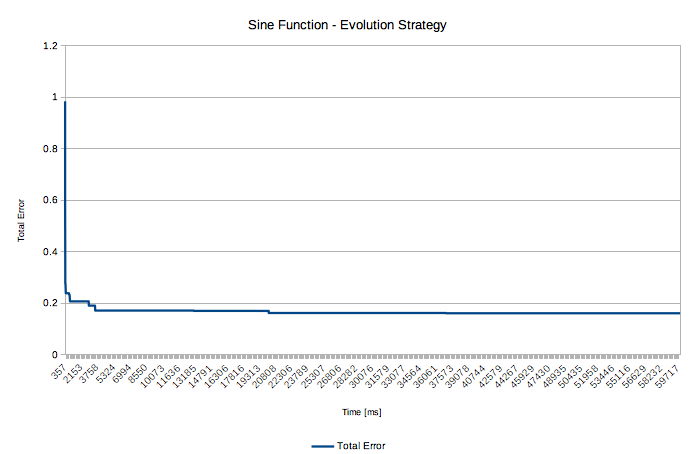
\includegraphics[width=0.8\linewidth]{fig0094.png}
  \caption{Еволюционна стратегия върху синус функция}
\label{fig0094}
\end{figure}

Синус функцията дава относително опростен времеви ред и резултатите показват сходимост на процеса по обучението на изкуствената невронна мрежа с алгоритъма за еволюционна стратегия (Фиг. \ref{fig0094}).

\newpage

\begin{figure}[H]
  \centering
  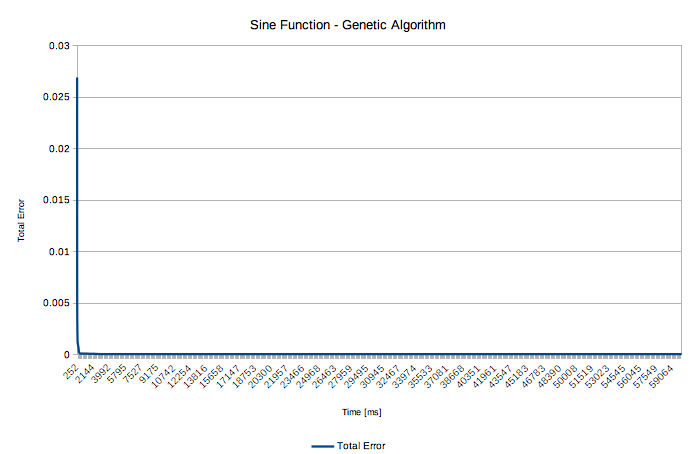
\includegraphics[width=0.8\linewidth]{fig0095.png}
  \caption{Генетичен алгоритъм върху синус функция}
\label{fig0095}
\end{figure}

Генетичният алгоритъм също дава сходимост при първите итерации от обучението на изкуствената невронна мрежа (Фиг. \ref{fig0095}).

\begin{figure}[H]
  \centering
  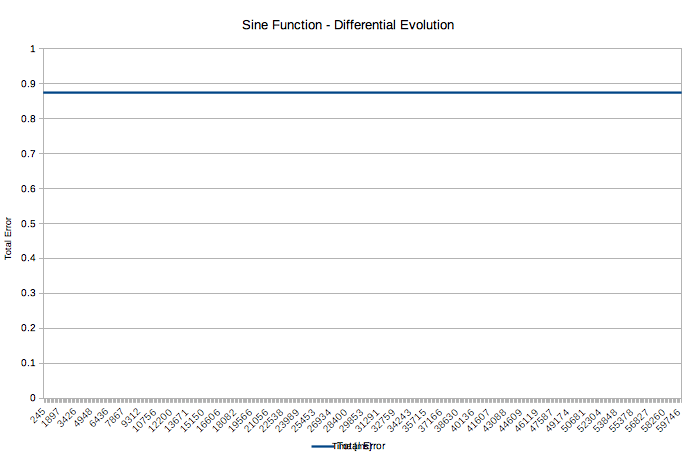
\includegraphics[width=0.8\linewidth]{fig0096.png}
  \caption{Еволюция на разликите върху синус функция}
\label{fig0096}
\end{figure}

При еволюцията на разликите не се забелязва подобрение в резултатите от оптимизационния процес (Фиг. \ref{fig0096}). Това се дължи на факта, че алгоритъмът не успява да излезе от локалния оптимум, в който попада още след първата оптимизационна итерация. 

\subsection{Цена на биткойн}

\begin{figure}[H]
  \centering
  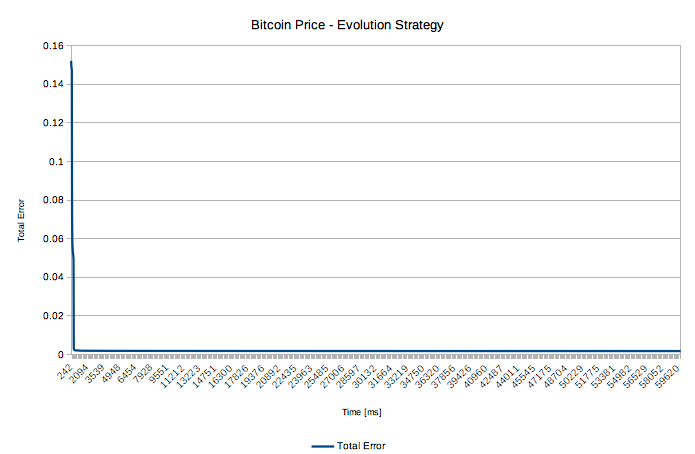
\includegraphics[width=0.8\linewidth]{fig0097.png}
  \caption{Еволюционна стратегия върху цена на биткойн}
\label{fig0097}
\end{figure}

Времевият ред с цената на дигиталната валута биткойн, отразена в щатски долари, е значително по-сложен като структура. От една страна, има много повече отчетени стойности, но също така формата е доста по-сложна. Въпреки това, еволюционната стратегия показва ясна сходимост (Фиг. \ref{fig0097}).

\begin{figure}[H]
  \centering
  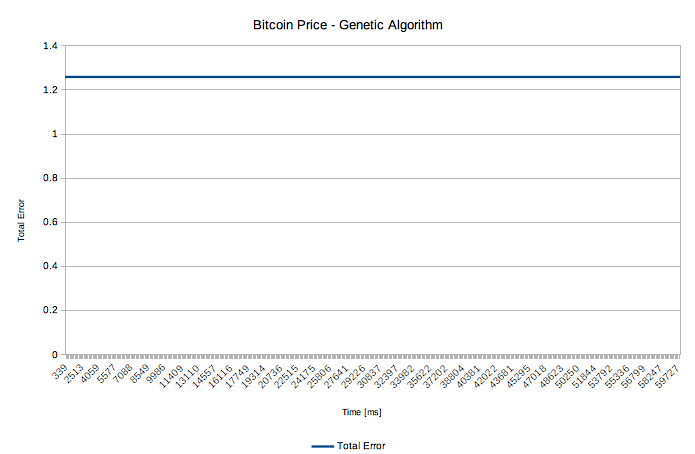
\includegraphics[width=0.8\linewidth]{fig0098.png}
  \caption{Генетичен алгоритъм върху цена на биткойн}
\label{fig0098}
\end{figure}

При по-сложен времеви ред, генетичният алгоритъм изпада в локален опитимум още след първата итерация (Фиг. \ref{fig0098}), по аналогия с еволюцията на разликите в по-опростения времеви ред.

\begin{figure}[H]
  \centering
  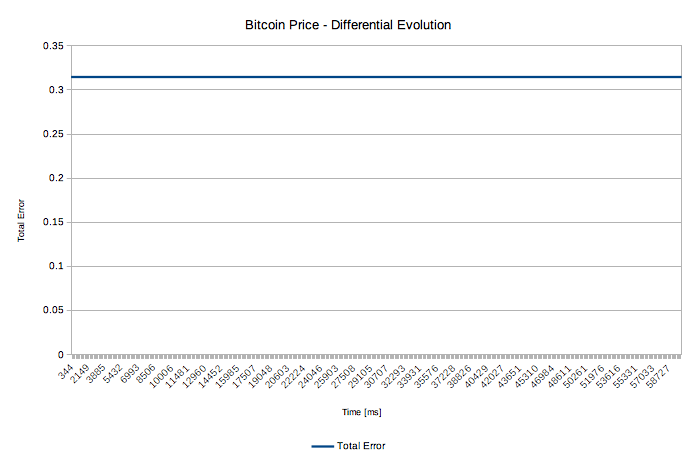
\includegraphics[width=0.8\linewidth]{fig0099.png}
  \caption{Еволюция на разликите върху цена на биткойн}
\label{fig0099}
\end{figure}

Еволюцията на разликите показва същото поведение, което бе отчетено и при по-опростения времеви ред (Фиг. \ref{fig0099}).

\subsection{Анализ на ефективността}

От резултатите след проведените експерименти, ясно се вижда, че алгоритъмът за еволюционна стратегия работи ефективно, както при по-опростени времеви редове, така и при по-сложни времеви редове. При по-опростени времеви редове, генетичните алгоритми показват сходимост, но при по-сложни времеви редове са недостатъчно ефективни. Еволюцията на разликите не показва признаци за сходимост, както при по-опростени времеви редове, така и при по-сложни. Определена ефективност на генетичните алгоритми и еволюцията на разликите може да се очаква при по-продължително време за работа и в ситуации, когато вече има попадане в локален опитимум. 

При проведените експерименти, параметрите на различните евристични алгоритми са избрани със стойности по подразбиране, но в реална работна среда, параметрите се избират с помощта на случайно търсене. Възможно е да се доразработи адаптивна стратегия за подбор на най-ефективните стойности за параметрите на евристичните алгоритми, но това изследване попада извън обхвата на настоящия труд и е въпрос на бъдещи изследвания. 

\section{Обобщение}

Изпълнен е сравнителен анализ на подбраните точни числени и евристични алгоритми за обучение на изкуствени невронни мрежи. При точните числени алгоритми ясно се откроява обучението с обратно разпространение на грешката. Получените резултати са представени в \cite{Tomov-08}. При евристичните алгоритми добри резултати показва обучението с еволюционна стратегия.

\begin{lstlisting}[caption=Случаен избор на точните числени алгоритми, language=Java, basicstyle=\tiny, label=list0023]
propagation = propagations[PRNG.nextInt(propagations.length)];
\end{lstlisting}

Макар и някои от използваните алгоритми за обучение да не дават твърде голяма ефективност, те могат да дадат допълнително разнообразие в генетичния фонд на еволюционните алгоритми, които са в хибридна употреба с точните числени алгоритми. Всеки от петте точни числени алгоритъма бива избиран на случаен принцип, равно вероятно, за участие в обучението (Листинг \ref{list0021} и \ref{list0023}). Обучението на изкуствената невронна мрежа не започва от случайно подбрани тегла, а продължава от там, до където е стигнато при предишна обучаваща сесия. 

